The core principles of the SmartSoft Architecture will be pointed out in the following
sections. A general overview of how components work together with the \textit{Sequencer} and the \textit{Instruction Planner} will be discussed,
as well as the deployment of the software components (which computer runs which software components and how these are connected).

\section{SmartSoft}
Before the software architecture of the RoboCup project is discussed, the SmartSoft approach is explained in a very brief way. Detailed information about SmartSoft can be found at the project homepage \url{http://www.servicerobotik-ulm.de/} and also in \cite{JOSER}.\\
SmartSoft is a model-driven software development approach (MDSD) for service robotic systems. It follows a strict separation-of-roles principle, which divides the development process into different responsibilities, like component development, application building and the end user. It combines via predefined communication patterns distributed components to complex scenarios.
With SmartSoft, typical 3-layer architectures can be realized (see figure \ref{fig:architecture_smartsoft_layers}), where a sequencing layer is responsible for orchestrating task execution. It involves a deliberative layer for task planning where required.

\begin{figure}[h]
\centering
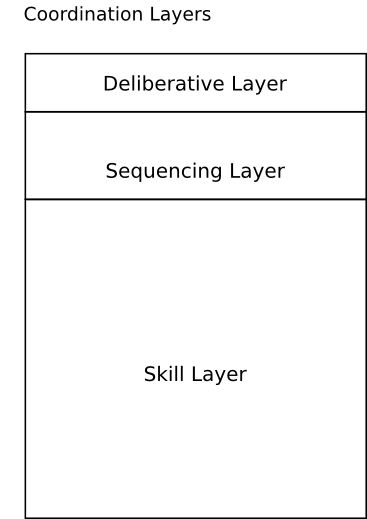
\includegraphics[scale=1.0]{pic/coordination_layers_smartsoft.png}
\caption{Coordination Layers of SmartSoft, Source: \protect\url{http://www.servicerobotik-ulm.de/drupal/?q=node/86}}
\label{fig:architecture_smartsoft_layers}
\end{figure}

The general idea is that basic capabilities are located in software components in the Skill Layer (e.g. Docking, Detection, LaserScan, ...). The Sequencing Layer monitors the situation of the task execution, including coordinating and configuring all other software components in the system. The Deliberative Layer reasons about the high-level goals of the system by using analysis tools, symbolic task planner, constraint solver, etc..

The following figure \ref{fig:architecture_overview} shows the basic architecture of the deployed software on the robots, which are involved in the RoboCup. \\

\begin{figure}[h]
\centering
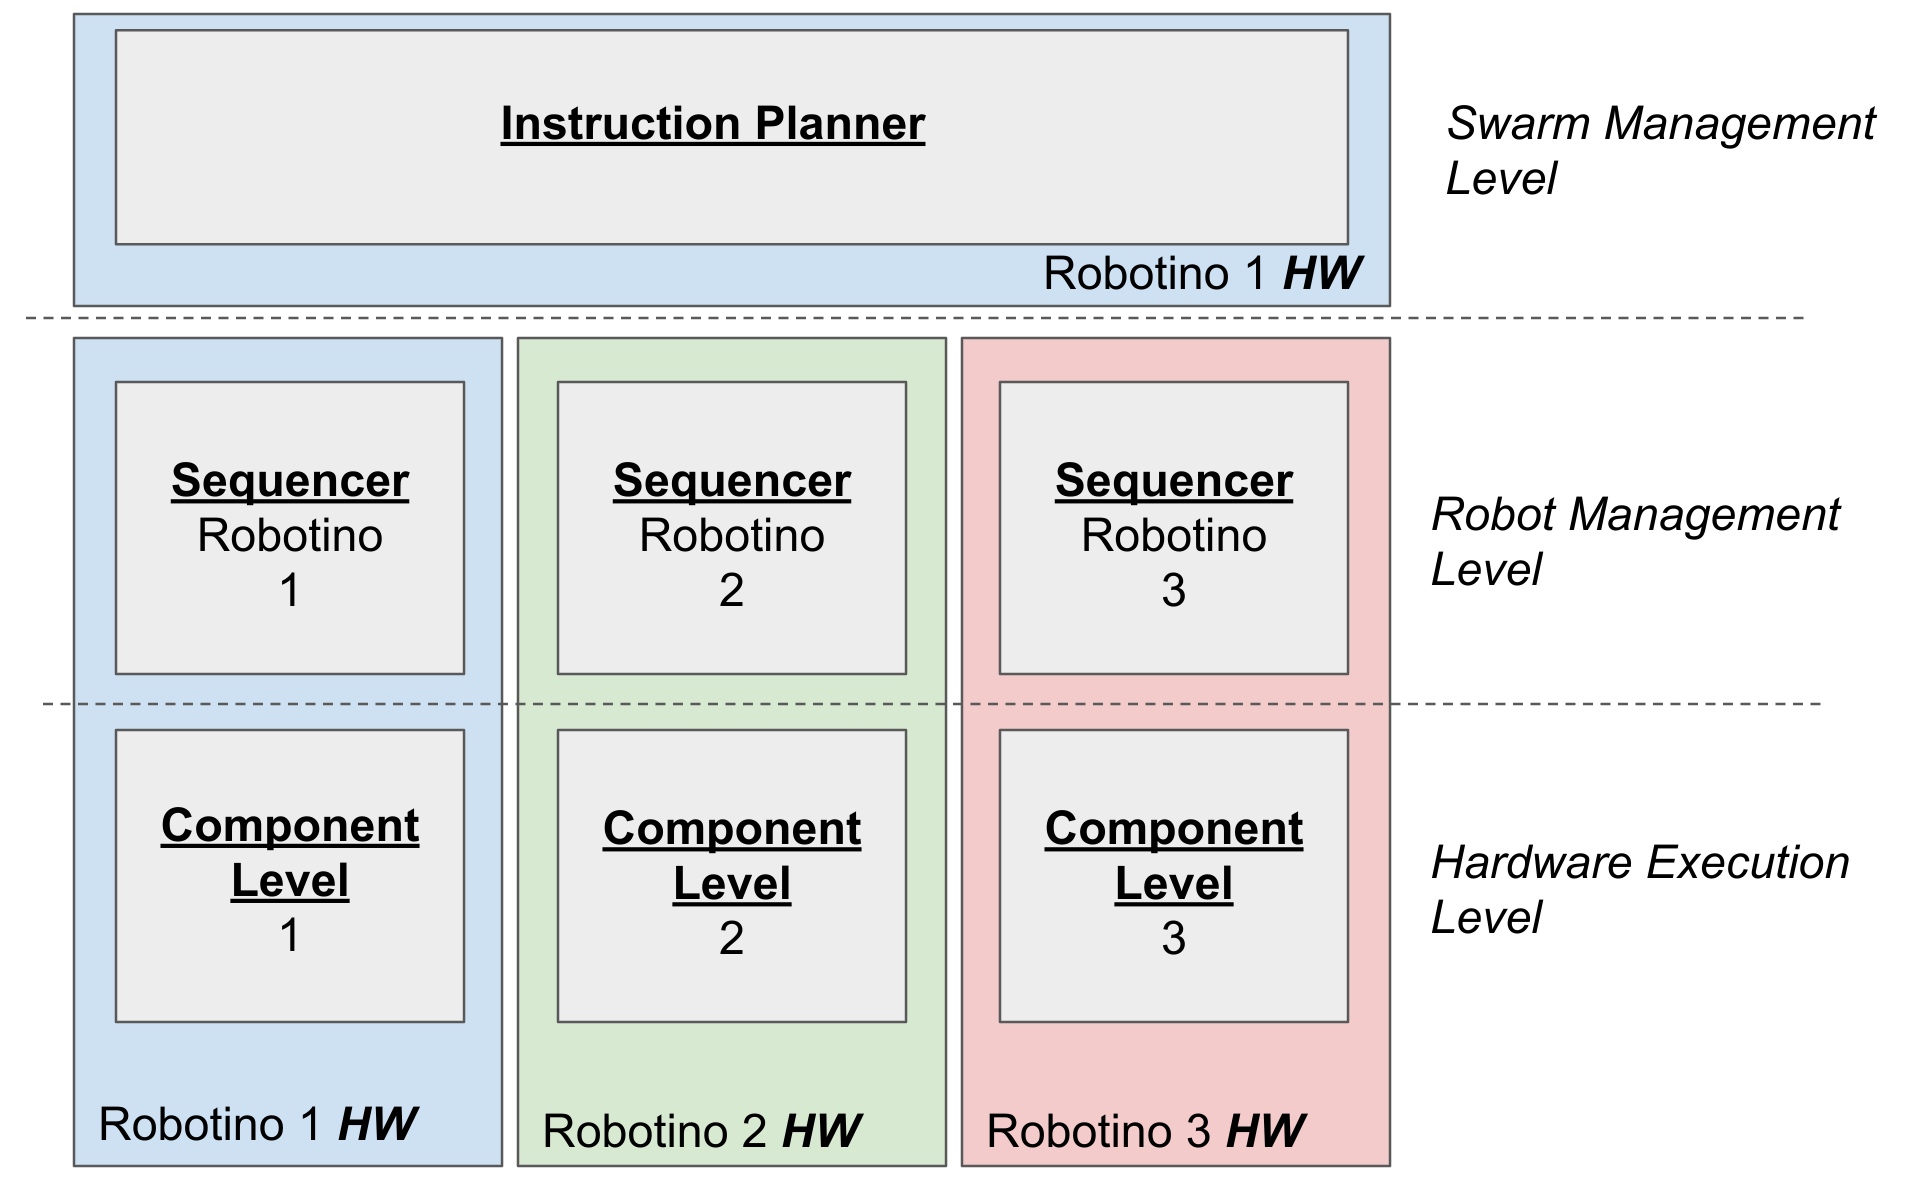
\includegraphics[scale=0.23]{pic/architecture2018.png}
\caption{Arrangement of Components in Architecture}
\label{fig:architecture_overview}
\end{figure}

As seen in figure \ref{fig:architecture_overview}, some parts of the system run as a copy on every robot (e.g. the Sequencer or movement dependent components), and the Instruction Planner is unique in the complete RoboCup scenario. The details of the different components are described in chapter \ref{ch:components}. The following subchapters give a short description of the involved parts.

\subsection{Instruction Planner}
The Instruction Planner takes care that the task assigned to the robotic system will be handled in an effective way. It consists of two parts, the \textbf{Fleet Management} and the \textbf{Objective Management} (see section \ref{ch:SmartRobotinoInstructionPlanner}). \\
\\
It actually does not matter on which machine the \textit{Instruction Planner} is deployed, it can be an external computer, or just one of the robots that are deployed on the field.\\
The limitation is that the \textit{Instruction Planner} has to:
\begin{itemize}
    \item have a stable connection to all other robots and to the Refbox
    \item be singular
\end{itemize}
Especially the need for being singular is one point that has to be considered in further progress of the system.
\\
The purpose of the Instruction Planner is to keep track of both the course of the game and the robots that are participating.
Based on the information that is provided by all the robots, the Instruction Planner decides which robot has to perform which task.

\subsection{Sequencer}
The Sequencer is often referred to as the \textit{"LispServer"} and manages the events that locally occur on the robot. The purpose of the Sequencer is to coordinate the overall behavior 
of a robot. 
A good example is the collision free movement: The robots are able to approach a position on the field without hitting objects in their way. For this, a coordination and configuration of different components is needed, 
e.g. the \textit{Laser scanner} and the \textit{Moving components}. This is done by the Sequencer. The Sequencer receives events from the involved components and orchestrates them.

\subsection{Components}
Skills are the most low level implementations of tasks (e.g. the handling of the movement of the wheels, docking to machines, detection of machines, etc.).
Also all other mentioned parts, as the Sequencer or the Instruction Planner are also components which can be deployed.
All these components communicate with each other using events that are delegated by the Sequencer.
The purpose of the components is the interface to the hardware or software that they handle.
Based on actual sensor values and information delegated by the Sequencer, skills fulfill only very fine granular tasks. Components can be composed, even dynamically, to very different systems.

\subsection{Deployments}
\label{subsec:Deployments}
Deployments are the connection of all needed components.
A Deployment mostly consists of a map (model driven - code is generated) that describes the connections between all components.
A deployment runs a scenario on a robot (e.g. Robocup - Exploration Phase).

\section{RoboCup specifics}
The RoboCup setup consists of three robots of type Festo Robotino 3 (called Robotinos) and the Referee Box (called Refbox).

\subsection{Robots}
The Robots are the Festo Robotinos, that are equipped with multiple hardware extensions to be able to sense and act
in an industrial (or other indoor) environments.\\
The hardware includes:
\begin{itemize}
    \item \textbf{Camera - LOGITECH HD Pro C920} - to perform the tag detections
    \item \textbf{Laserscanner - SICK LMS-100} - to sense the environment for objects
    \item \textbf{Gripper -  not specified} - to be able to move the products around% [\textit{needed in Production phase}]
    \item \textbf{5Ghz Wireless LAN} - to communicate with the refbox and other robots
\end{itemize}

The Robotino runs on a Ubuntu 16.04 LTS and can be accessed via VNC / HTTP / SSH.\\

The Robotino is the standard platform that every participant of the RoboCup has to work with.\\
In the contest all Robotinos will be connected to the Refbox and listen for its signals to start the given phases.
The rest of the communication will be performed in a team channel where the Robotinos can exchange messages to each other.
\newpage

\subsection{Referee Box}
The Refbox is the master of the game, and is controlled by a human referee. It takes care of the game progress, as well as the awarding of points and the disqualification of robots.
The Refbox also works event based, so it is bursting out events of the game state (e.g. start / stop or game phases) and receives the messages of the robots to score their points.
It is also always in contact with all of the robots to ensure that they obey the rules.
